% !TeX root = ../main.tex

\chapter{结果与结论}

\section{结果}

对于尺寸为256x256的视频输入,两种方法处理前10帧画面的时间如图 \ref{fig:time-frame} 所示。
其中方法一表示使用TorchScript工具将模型导出,在C++前端直接调用模型;方法二是使用LibTorch将神经网络重新构建为类对象,在C++前端把类对象实例化。
可以看出,方法一(蓝色)在处理前两帧画面时花费的时间较久,第一帧花费 250 ms,第二帧则需要 1000 ms,之后稳定在 84 ms。
方法二(橙色)第一帧花费 120 ms,第二帧需要 100 ms,之后稳定在 86 ms。至于原因可能涉及到 TorchScript 底层代码的实现,暂未得知。

由于两种方法的网络权重参数均是从同一个文件中加载,因此输出的图像完全相同。

\begin{figure}[h]
\centering
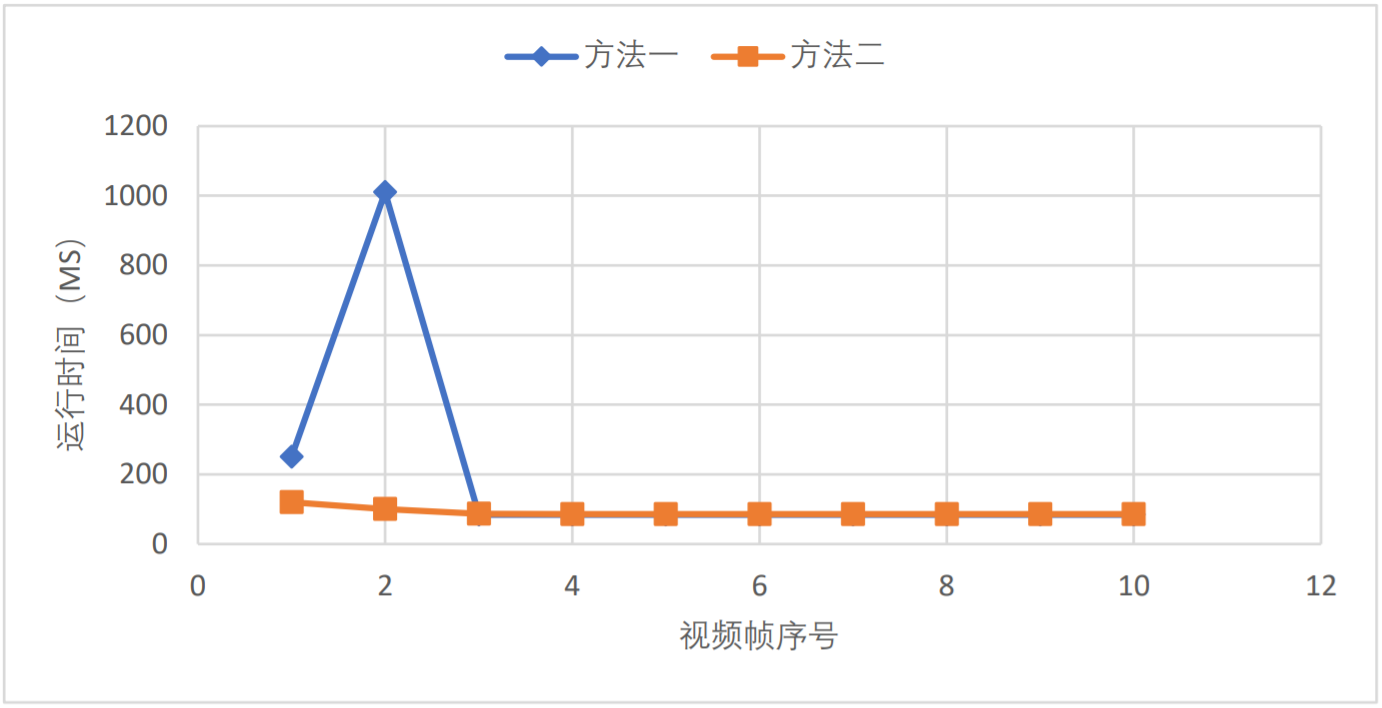
\includegraphics[width=0.8\textwidth]{time-frame.PNG}
\caption{前10帧画面运行时间}
\label{fig:time-frame}
% \note{注:图注的内容不宜放到图题中。}
\end{figure}

\section{分析}

每帧图像的处理时间主要与网络结构深度和输入图像尺寸有关。如图 \ref{fig:time_a},对于固定尺寸的输入,随着神经网络深度的加深,处理时间几乎是线性增长;
另一方面,如图 \ref{fig:time_b},对于固定深度的神经网络,随着输入尺寸的增加,处理时间也在逐渐增长。对于本文中嵌入的网络PoolNet来说,其卷积层数为92,
输入尺寸大小为256x256,因此每帧处理时间较慢。

\begin{figure}[h]
    \centering
    \begin{subfigure}{.4\textwidth}
        \centering
        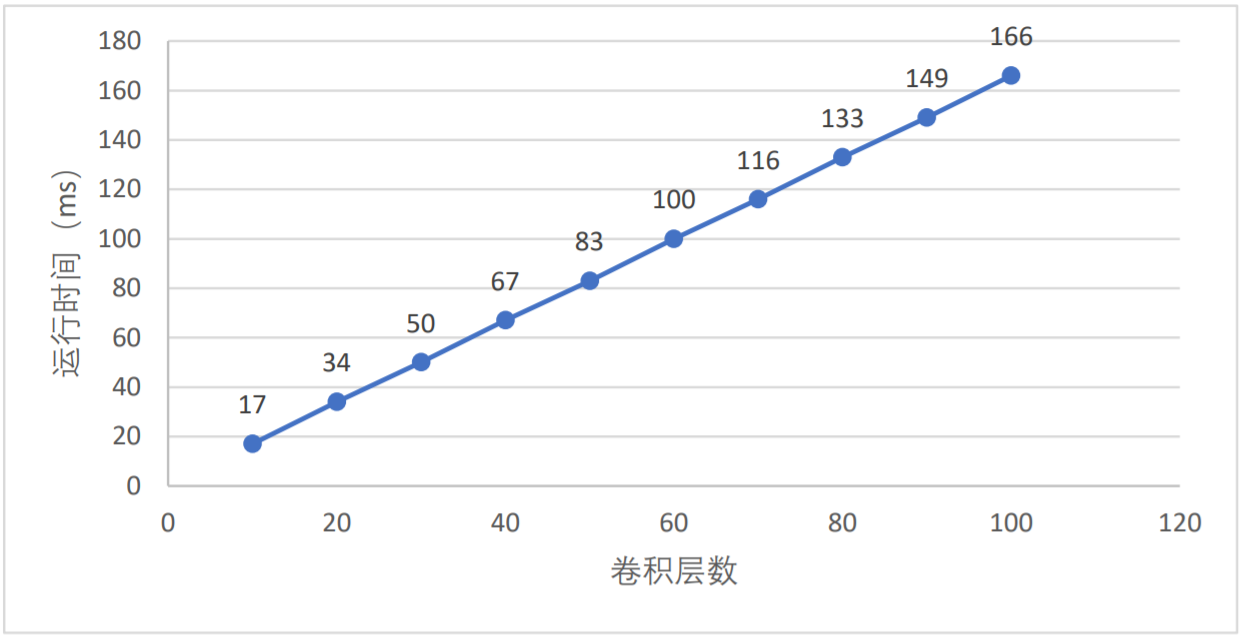
\includegraphics[width=\textwidth]{time-depth.PNG}
        \caption{处理时间与卷积层数的关系。}
        % \note{注:图注的内容不宜放到图题中。}
        \label{fig:time_a}
    \end{subfigure}
    \begin{subfigure}{.4\textwidth}
        \centering
        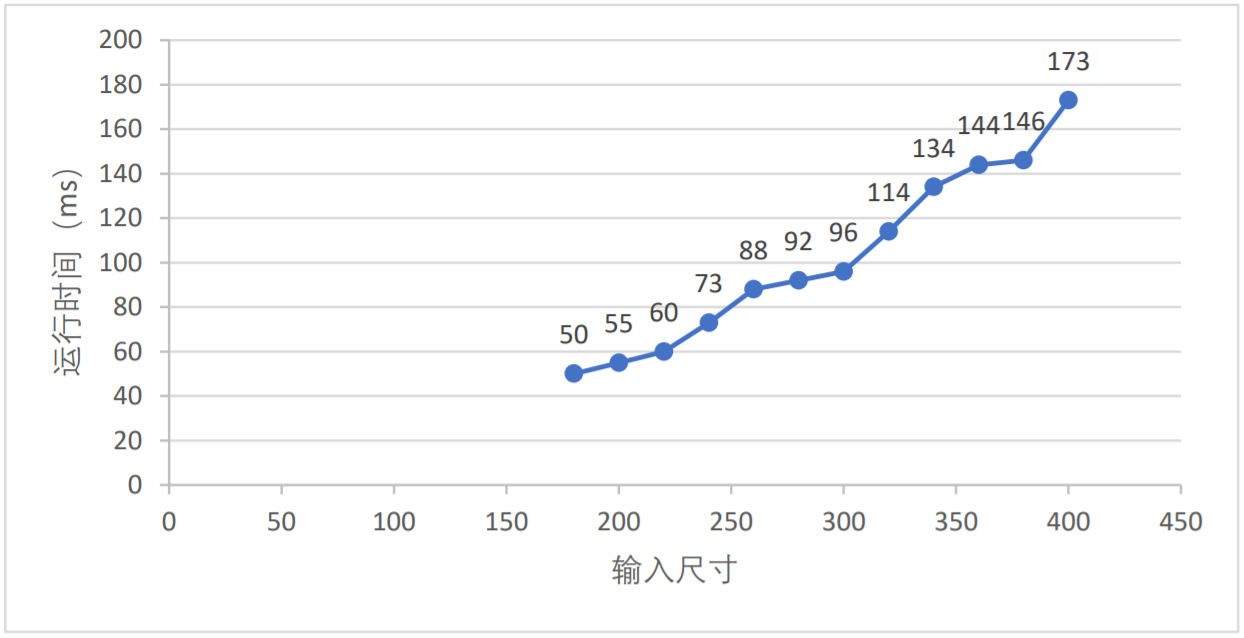
\includegraphics[width=\textwidth]{time-input.PNG}
        \caption{处理时间与输入尺寸的关系。}
        % \note{注:图注的内容不宜放到图题中。}
        \label{fig:time_b}
    \end{subfigure}
    \caption{处理时间的影响因素}
    \label{fig:time}
\end{figure}

人眼识别连贯图像的速度是每秒24帧,也就是说每帧处理的时间应低于40ms。就目前的256x256的输入来看,每帧的处理时间只能达到84ms,人眼观看视频时
会有明显的卡顿。虽然可以尝试缩小图像尺寸以缩短运行时间,但是像素数据的丢失会导致显著性检测算法难以捕捉全局信息。如图 \ref{fig:result} 所示,
随着图片尺寸的缩小,运行效果越来越差。

\begin{figure}[h]
    \centering
    \begin{subfigure}{.1\textwidth}
        \centering
        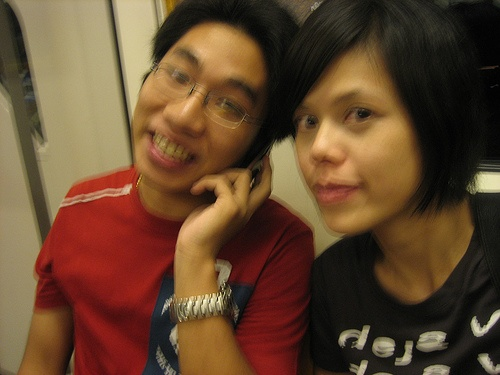
\includegraphics[width=\textwidth]{2007_000323.jpg}
        \centering
        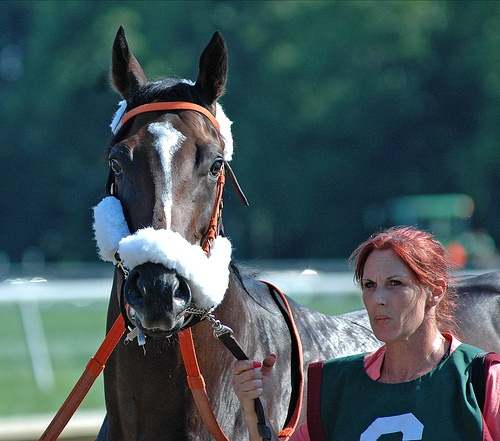
\includegraphics[width=\textwidth]{2007_000799.jpg}
        \centering
        
\includegraphics[width=\textwidth]{2007_000346.jpg}
        \caption{原图}
        % \note{注:图注的内容不宜放到图题中。}
    \end{subfigure}
    \begin{subfigure}{.1\textwidth}
        \centering
        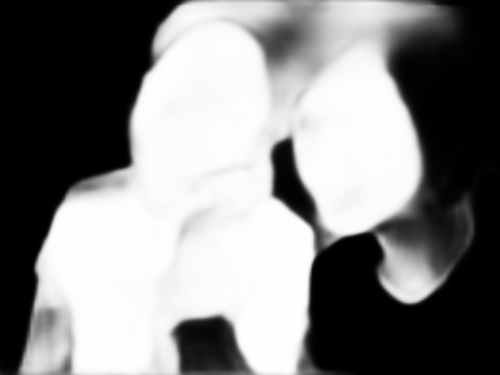
\includegraphics[width=\textwidth]{2007_000323_260.png}
        \centering
        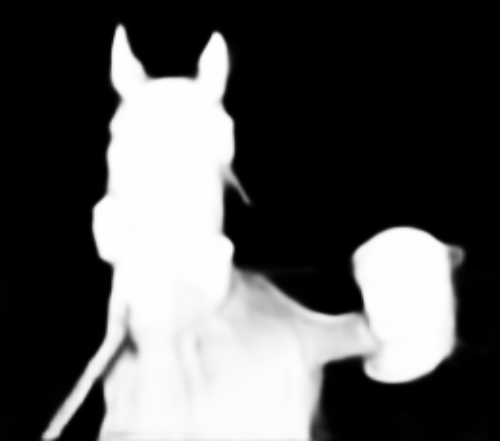
\includegraphics[width=\textwidth]{2007_000799_260.png}
        \centering
        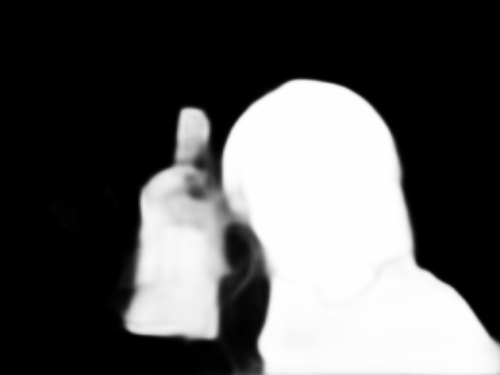
\includegraphics[width=\textwidth]{2007_000346_260.png}
        \caption{260}
        % \note{注:图注的内容不宜放到图题中。}
    \end{subfigure}
    \begin{subfigure}{.1\textwidth}
        \centering
        
\includegraphics[width=\textwidth]{2007_000323_240.png}
        \centering
        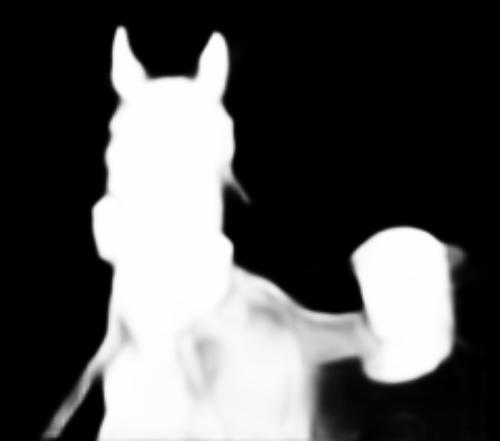
\includegraphics[width=\textwidth]{2007_000799_240.png}
        \centering
        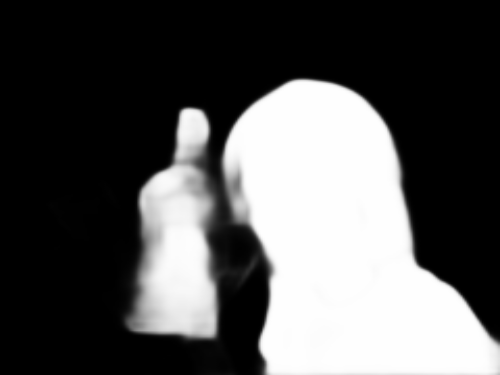
\includegraphics[width=\textwidth]{2007_000346_240.png}
        \caption{240}
        % \note{注:图注的内容不宜放到图题中。}
    \end{subfigure}
    \begin{subfigure}{.1\textwidth}
        \centering
        
\includegraphics[width=\textwidth]{2007_000323_220.png}
        \centering
        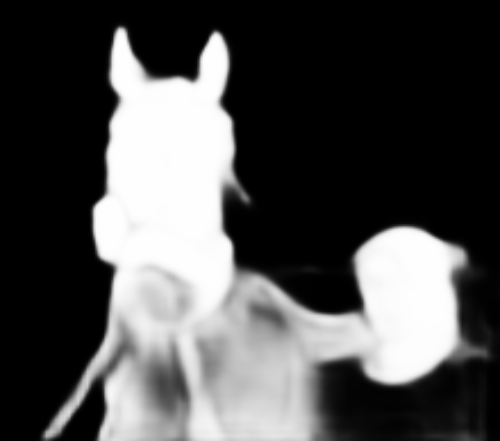
\includegraphics[width=\textwidth]{2007_000799_220.png}
        \centering
        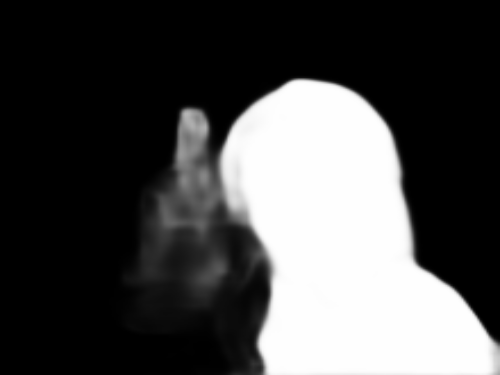
\includegraphics[width=\textwidth]{2007_000346_220.png}
        \caption{220}
        % \note{注:图注的内容不宜放到图题中。}
    \end{subfigure}
    \begin{subfigure}{.1\textwidth}
        \centering
        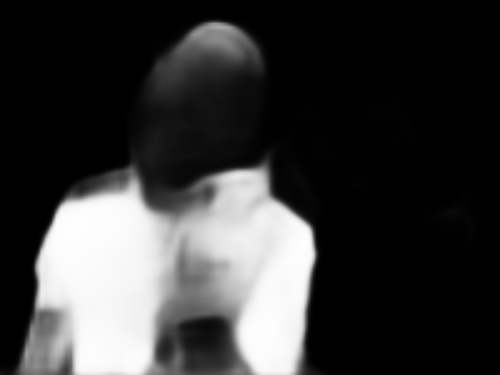
\includegraphics[width=\textwidth]{2007_000323_200.png}
        \centering
        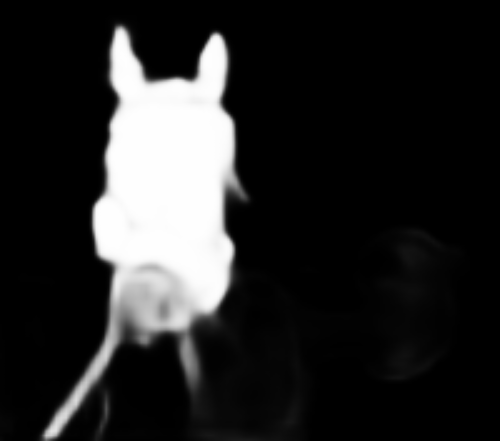
\includegraphics[width=\textwidth]{2007_000799_200.png}
        \centering
        
\includegraphics[width=\textwidth]{2007_000346_200.png}
        \caption{200}
        % \note{注:图注的内容不宜放到图题中。}
    \end{subfigure}
    \begin{subfigure}{.1\textwidth}
        \centering
        
\includegraphics[width=\textwidth]{2007_000323_180.png}
        \centering
        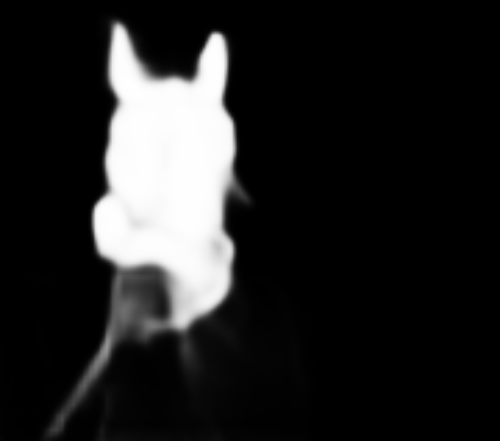
\includegraphics[width=\textwidth]{2007_000799_180.png}
        \centering
        
\includegraphics[width=\textwidth]{2007_000346_180.png}
        \caption{180}
        % \note{注:图注的内容不宜放到图题中。}
    \end{subfigure}
    \caption{缩小尺寸后的运行结果}
    \label{fig:result}
\end{figure}

\section{总结与展望}

为了增加FFmpeg对基于神经网络的图像处理算法的支持,
本文尝试了将显著性检测算法嵌入到FFmpeg的播放工具ffplay中并单独编译ffplay的方法,并介绍了两种调用神经网络的方式。由于神经网络深度和
输入尺寸的限制因素,算法每帧的处理时间达到84ms,帧率为12fps左右。本次实验存在下面几点不足,可以继续探究和改进。

第一点,PoolNet 在 pytorch 环境下,对于 300x400 的输入可以达到 30fps。但是,在 C++ 环境下,对于 256x256 的输入,
仅能达到 12fps。可以继续深入探究产生这种差别的原因。

第二点,实验室中的设备有 3 颗 GPU,但运行时仅使用一颗。之后可以尝试将图像切分,使用多颗 GPU 并行处理,然后再把结果合在一起。理论上这样
可以加快处理时间。

第三点,本文的工作是将神经网络算法嵌入到FFmpeg的播放工具ffplay中,虽然方便测试并且能够运行,但是不够灵活,导致ffplay的功能比较单一。
之后可以考虑把多种不同的神经网络算法集成到FFmpeg的滤镜功能中,从而根据不同的目的,使用对应的命令行参数调用对应的算法,更加方便灵活。